\section{Технологическая часть}
\subsection{Выбор средств программной реализации}
\subsubsection{Основные средства}
В качестве языка программирования был выбран Python 3 \cite{python}, ввиду \, нескольких причин.
\begin{itemize}
	\item Текущая работа подразумевает активное взаимодействие с ЕЯ, в частности, с русским языком, поэтому необходимы средства, позволяющие обрабатывать соответствующие тексты. На Python написано большое количество библиотек для NLP (Natural Language Processing -- обработка естественного языка).
	\item Также язык поддерживает объектно-ориентированный подход, что важно, поскольку в процессе реализации подразумевается использование этой методологии, позволяющей разрабатывать хорошо организованную \, и \, просто модифицируемую структуру приложения.
	\item Кроме того, предоставляются библиотеки для создания графического интерфейса, визуализации графов, которые планируется использовать для отладки и наглядной демонстрации работы приложения.
	\item В дополнение, в процессе обучения был накоплен существенный опыт в использовании этого языка программирования. \newline
\end{itemize}
%
В качестве среды разработки был выбран PyCharm \cite{pycharm} в силу следующих факторов.
\begin{itemize}
	\item Она бесплатна для студентов.
	\item Предоставляются удобные инструменты для написания, редактирования кода, а также графический отладчик.
	\item Помимо этого, является хорошо знакомой средой разработки, и какие-либо проблемы с взаимодействием сведены к минимуму, что позволяет сэкономить время.
\end{itemize}

\subsubsection{Вспомогательные средства}
Для сбора датасета использовалась кроссплатформенная система мгновенного обмена сообщениями Discord \cite{discord}. Это было сделано по следующим причинам.
\begin{itemize}
	\item Она бесплатна для всех пользователей.
	\item Поскольку необходимо было опросить большое количество людей, встречаться лично было затруднительно, поэтому гораздо удобнее и проще организовать весь процесс дистанционно, что и позволяет сделать это приложение.
	\item Платформа очень популярна среди молодых людей, что доказывает недавнее исследование от апреля 2022 года \cite{discordS}. Это упрощает поиск удобной большинству среды. 
	\item Для этой системы возможно написание дополнительного API в \, виде \, discord-бота, который может выполнять различные задачи. Так, для ускорения процесса фиксации слов опрашиваемых было создано дополнительное приложение, которое в реальном времени переводит речь участников в текст, заносит всю информацию в файлы и по каждому человеку создаёт базу знаний.
\end{itemize}

Для создания описанного выше discord-бота c заявленными функциями использовался язык Javascript \cite{javascript}, поскольку в основном для написания подобных приложений используют его, к тому же бОльшая часть кода Discord написана на этом языке программирования.\newline

\subsection{Используемые библиотеки}
Для разработки графического пользовательского интерфейса привлекалась библиотека PyQt5 \cite{pyqt5}. Qt -- один из самых популярных кроссплатформенных графических фреймворков \cite{qt}, поэтому кроме документации, описано множество примеров его использования. Для наглядной разработки GUI привлекалась среда Qt Designer \cite{qtdesigner}.

Для упрощения контроля над тем, правильно ли формируются графы и сети, используется библиотека NetworkX \cite{networkx}, позволяющая визуализировать подобные структуры. 

В приложении и discord-боте для перевода речи пользователя в текст используется библиотека Speech Recognition \cite{speech_rec}. Это инструмент от таких компаний, как Google, Microsoft, IBM и др. Для работы используется стандартный Google Speech API.

К другой библиотеке, Natasha \cite{natasha}, происходит обращение с целью выделения словосочетаний в предложениях. Natasha позволяет  с помощью готовых правил решать базовые задачи NLP для русского языка такие, как:
\begin{itemize}
	\item токенизация;
	\item сегментация;
	\item определение морфологических признаков;
	\item лемматизация/нормализация;
	\item выделение словосочетаний и т.д.
\end{itemize}

Кроме того, привлекается библиотека SciPy \cite{scipy}, которая ориентирована на работу с большим количеством данных, содержит много функций линейной алгебры, интерполяции, масштабирования данных. \newline

\subsection{Сбор данных для формирования онтологии}
Для сбора различных формулировок определений терминов был проведён устный опрос среди студентов как третьего курса бакалавриата, так и некоторых аспирантов кафедры <<Комбинированные двигатели и альтернативные энергоустановки>> факультета <<Энергомашиностроение>> с последующим переводом речи в текстовый формат посредством использования заранее разработанного discord-бота.

В общей сложности было собрано около 800 определений. \newline

\subsection{UML-диаграммы}
\textbf{Компонент доступа к данным}

Доступ к данным реализован с помощью \, паттерна \, проектирования \, Repository. Соответствующая UML-диаграмма представлена на рисунке \ref{fig49:image}.
\begin{figure}[h!]
	\begin{center}
		{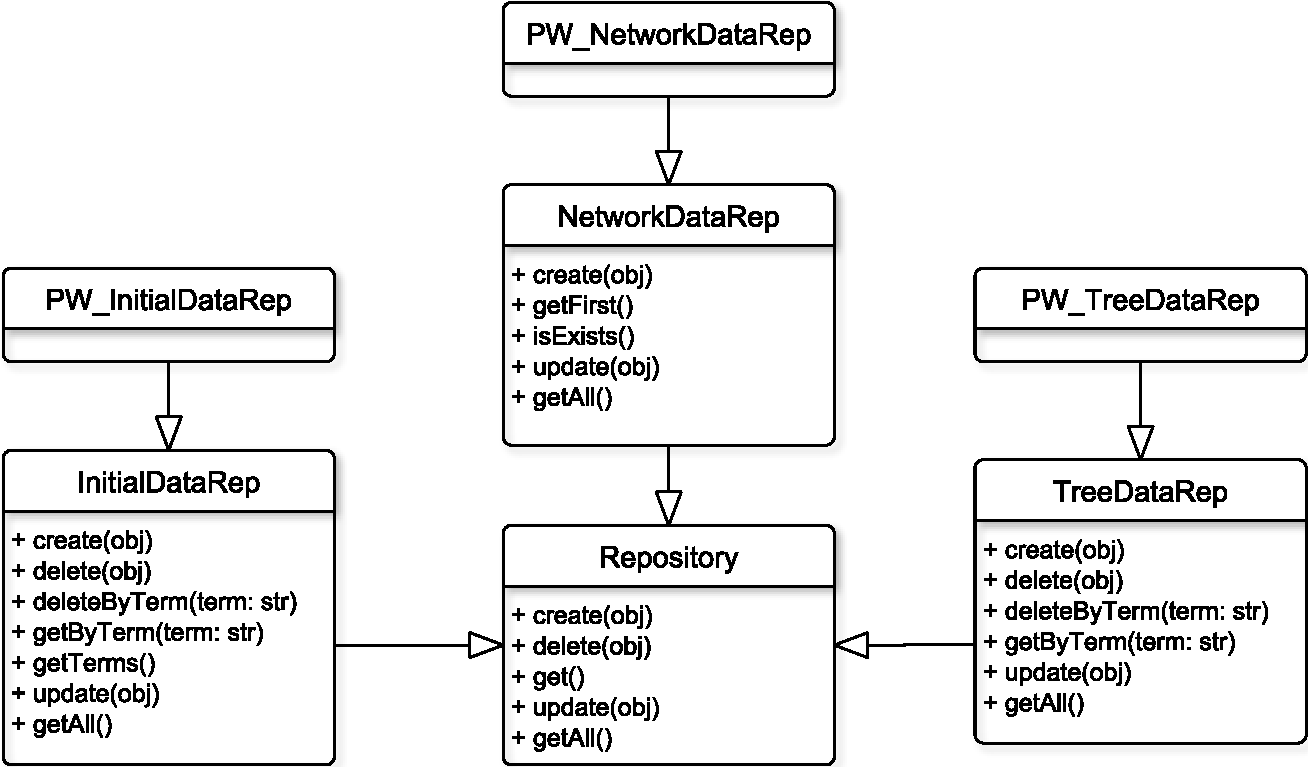
\includegraphics[scale = 0.6]{img/uml/pdf/uml_rep.pdf}}
		\caption{UML-диаграмма компонента доступа к данным.}
		\label{fig49:image}
	\end{center}
\end{figure}

\textbf{Компонент бизнес-логики}

Этот компонент выполняет основную обработку данных, соответствующая UML-диаграмма представлена на рисунке \ref{fig50:image}.
\begin{figure}[h!]
	\begin{center}
		{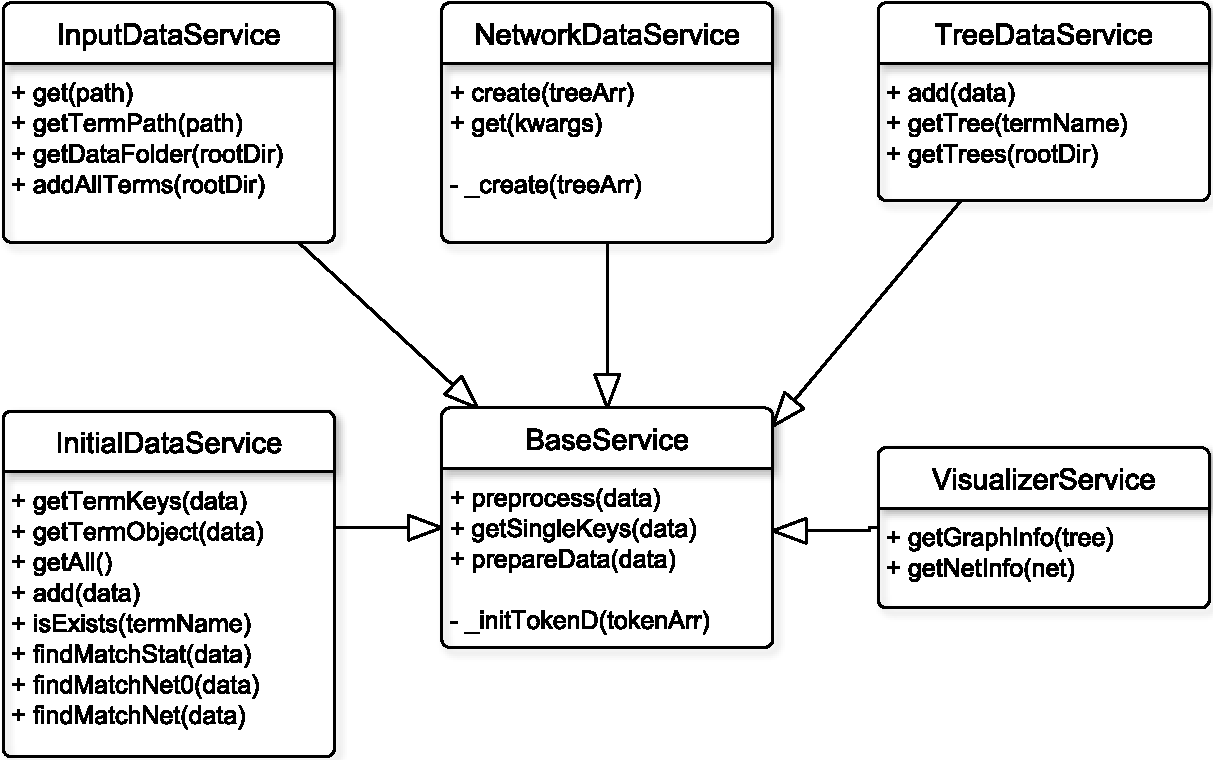
\includegraphics[scale = 0.6]{img/uml/pdf/uml_ser.pdf}}
		\caption{UML-диаграмма компонента бизнес-логики.}
		\label{fig50:image}
	\end{center}
\end{figure}

\newpage

\textbf{Компонент представления}

UML-диаграмма компонента, отвечающая за отображение, изображена на рисунке \ref{fig51:image}.
\begin{figure}[h!]
	\begin{center}
		{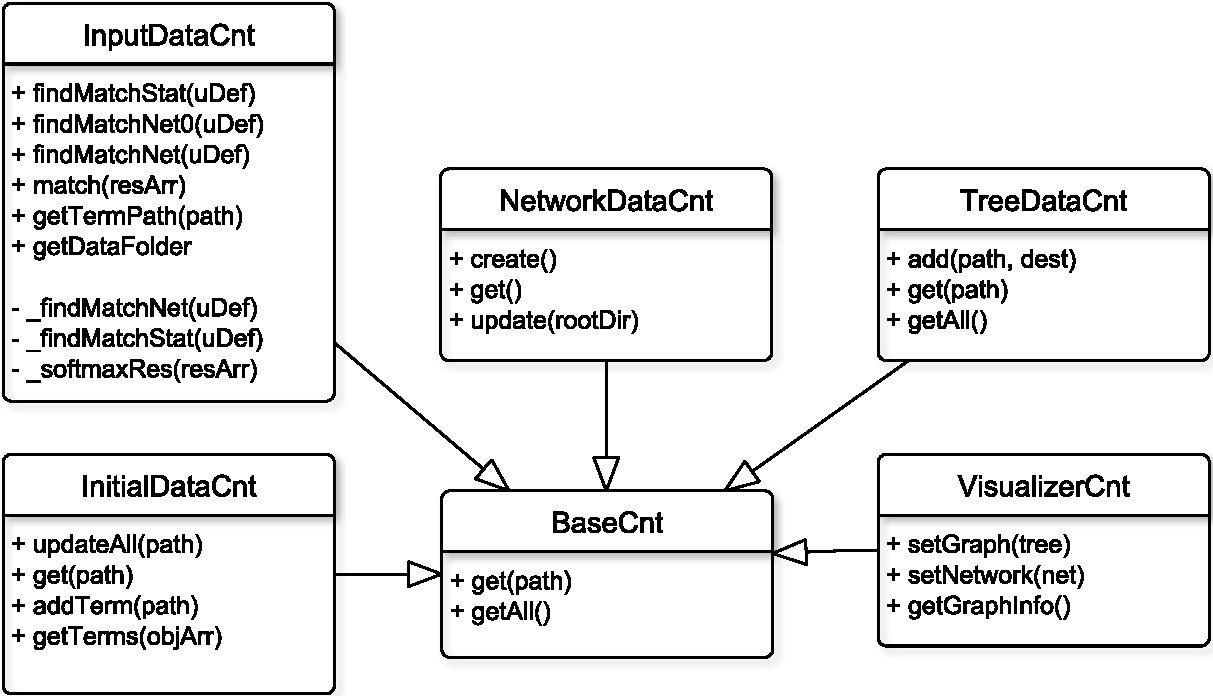
\includegraphics[scale = 0.6]{img/uml/pdf/uml_cnt.pdf}}
		\caption{UML-диаграмма компонента представления.}
		\label{fig51:image}
	\end{center}
\end{figure}


\subsection{Интерфейс программы}
На рисунках \ref{fig40:image}-\ref{fig42:image} представлен графический интерфейс пользователя.

Пользователь может ввести свой запрос в текстовое поле, либо воспользоваться голосовым вводом, нажав на кнопку микрофона. При нажатии на кнопку <<Готово>>, начнётся процесс поиска нечётких дубликатов, результат которого будет выведен в разделах <<Косинусное сходство>> и <<Сеть синтаксических графов>>.
\begin{figure}[h]
	\begin{center}
		{\includegraphics[scale = 0.5]{img/ui/ui1.png}}
		\caption{Графический интерфейс (администратор/пользователь).}
		\label{fig40:image}
	\end{center}
\end{figure}

Последующие две страницы приложения доступны только администратору. На рисунке \ref{fig41:image} изображёно окно для редактирования онтологий, помимо этого, нажав на кнопку графа в терминологическом отделе, можно увидеть как выглядит граф для выбранного термина.
\begin{figure}[h!]
	\begin{center}
		{\includegraphics[scale = 0.5]{img/ui/ui2.png}}
		\caption{Графический интерфейс (администратор).}
		\label{fig41:image}
	\end{center}
\end{figure}

\newpage

На рисунке \ref{fig42:image} представлен графический интерфейс посредством которого можно наглядно увидеть сеть для всей онтологии, а также ключевые определения терминов.
\begin{figure}[h]
	\begin{center}
		{\includegraphics[scale = 0.6]{img/ui/ui3.png}}
		\caption{Графический интерфейс (администратор).}
		\label{fig42:image}
	\end{center}
\end{figure}

\newpage

\subsection{Демонстрация работы программы}
Введём с помощью голосового ввода описание понятия <<сжатие>>: <<Как называется процесс уменьшение объёма>> (рисунок \ref{fig43:image}). 
\begin{figure}[h!]
	\begin{center}
		{\includegraphics[scale = 0.6]{img/examples/ex1_1.png}}
		\caption{Ввод данных.}
		\label{fig43:image}
	\end{center}
\end{figure}

Результат применения косинусного сходства представлен на рисунке \ref{fig44:image}. Наибольшее вычисленное расстояние -- с терминами <<сжатие>>, <<изохорный \, процесс>> (т.к. последний -- термодинамический процесс, происходящий при постоянном объёме).
\begin{figure}[h]
	\begin{center}
		{\includegraphics[scale = 0.6]{img/examples/ex1_2.png}}
		\caption{Результат поиска с помощью косинусного сходства.}
		\label{fig44:image}
	\end{center}
\end{figure}

Из-за того, что самый высокий процент меньше 50, то дополнительно осуществляется поиск по семантической сети. Результат представлен на рисунке \ref{fig45:image}.
\begin{figure}[h]
	\begin{center}
		{\includegraphics[scale = 0.6]{img/examples/ex1_3.png}}
		\caption{Результат с помощью сети синтаксических графов.}
		\label{fig45:image}
	\end{center}
\end{figure}

Несмотря на то, что при таком подходе процент ниже (около 40\%), в то же время у термина <<изохорный процесс>> он гораздо меньше, чем был ранее (только 15\%). Разработанный метод верно определил описываемый объект.

Если нажать на кнопку графа, то можно увидеть сеть, которая была построена конкретно для текущего запроса пользователя (рисунок \ref{fig46:image}).

У администратора есть возможность посмотреть синтаксические графы для любого из загруженных терминов, для этого следует нажать на кнопку графа во второй вкладке приложения (рисунок \ref{fig44:image}). Так, для термина <<термодинамический цикл>> синтаксический граф для определения: <<Термодинамический цикл -- непрерывная последовательность термодинамических процессов, в результате которых рабочее тело возвращается в исходное состояние>>, выглядит так, как показано на рисунке \ref{fig47:image}.
\begin{figure}[pt!]
	\begin{center}
		{\includegraphics[scale = 0.55, angle=90]{img/examples/ex1_4.png}}
		\caption{Построенная для рассматриваемого запроса сеть.}
		\label{fig46:image}
	\end{center}
\end{figure}

\newpage
\begin{figure}[t]
	\begin{center}
		{\includegraphics[scale = 0.6]{img/examples/tree.png}}
		\caption{Синтаксический граф для термина <<термодинамический цикл>>.}
		\label{fig47:image}
	\end{center}
\end{figure}
Также есть функция просмотра сети по всей онтологии, которая есть в базе данных. Её можно увидеть, нажав на соответствующую клавишу на третьей вкладке (рисунок \ref{fig42:image}). Результат представлен на рисунке \ref{fig48:image}.

\begin{figure}[h!]
	\begin{center}
		{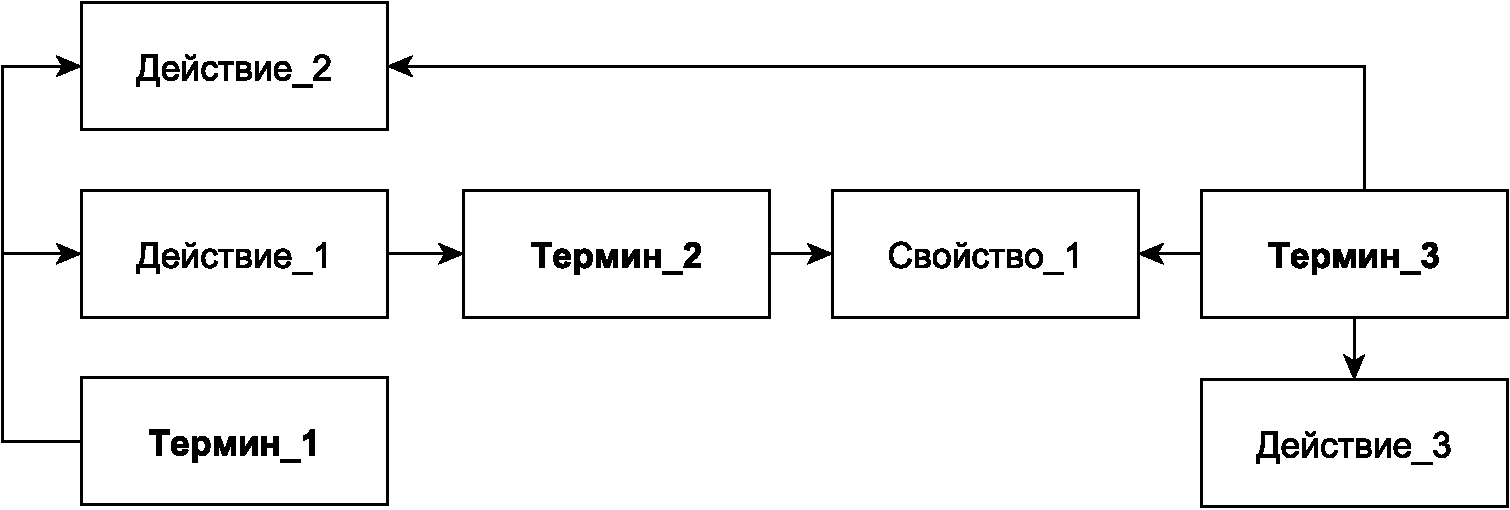
\includegraphics[scale = 0.52, angle=90]{img/examples/net.png}}
		\caption{Сеть по всей онтологии.}
		\label{fig48:image}
	\end{center}
\end{figure}

\newpage

\subsection{Тестирование программы}
Было проведено тестирование как методом чёрного ящика (таблица \ref{table_black}), так и модульное (таблица \ref{table_module}).

\begin{longtable}{|p{6cm}|p{5cm}|p{4.5cm}|}
	\caption{Тестирование методом чёрного ящика}\label{table_black}\\
	\hline
	
	\textbf{Описание} & \textbf{Примеры} & \textbf{Ожидаемый результат }\\ 
	\hline
	\endfirsthead
	
	\hline
	\textbf{Описание} & \textbf{Примеры} & \textbf{Ожидаемый результат }\\ 
	\hline
	\endhead
	
	\hline
	\multicolumn{3}{c}{\textit{Продолжение на следующей странице}}
	\endfoot
	\hline
	\endlastfoot
	
	\textbf{Вход}: определения, по которым создавалась онтология на базе статистических данных. &
	1. Уменьшение рабочего объема. & 
	1. Сжатие \\
	&&\\
	
	\textbf{Ожидаемый результат}: Наибольшее косинусное сходство у корректного термина. & 
	2. Цикл, протекающий как в одном, так и в обратном направлении, в замкнутой системе& 
	2. Обратимый цикл\\
	
	\hline
	\textbf{Вход}: определения из словаря терминов, проверяемая сущность -- сеть, созданная по всей онтологии. & 
	1. Процесс уменьшения объема рабочего тела посредством движения поршня к верхней мертвой точке & 
	1. Сжатие \\ 
	
	&&\\
	
	\textbf{Ожидаемый результат}: правильно определённый объект. &
	2. Термодинамический цикл, в котором все процессы являются обратимыми &
	2. Обратимый цикл\\
	
	\hline
	\textbf{Вход}: пустой ввод. & 
	1. (пустая строка) & 
	1. Сообщение об ошибке \\

	\textbf{Ожидаемый результат}: сообщение об ошибке. &
	&\\
\end{longtable}

\begin{longtable}{|p{6cm}|p{5cm}|p{4.5cm}|}
	\caption{Модульное тестирование}\label{table_module}\\
	\hline
	
	\textbf{Описание} & \textbf{Примеры} & \textbf{Ожидаемый результат }\\ 
	\hline
	\endfirsthead
	
	\hline
	\textbf{Описание} & \textbf{Примеры} & \textbf{Ожидаемый результат }\\ 
	\hline
	\endhead
	
	\hline
	\multicolumn{3}{c}{\textit{Продолжение на следующей странице}}
	\endfoot
	\hline
	\endlastfoot
	
	\hline
	\multicolumn{3}{|c|}{\textbf{Проверяется метод предобработки текста.}}
	\\
	\hline
	
	\textbf{Вход}: множество строк, включающих: 
	\begin{itemize}
		\item вводные фразы, междометия, слова из группы стоп-слов;
		\item цифры и символы;
		\item различное написание слов с буквами е и ё.		
	\end{itemize} &
	1. Я думаю, что это такой двигатель \newline
	2. Ой, это механизм для управления \newline
	3. В двигателе есть 2 специальные детали, которые управляют всем процессом!!!! \newline
	4. Объём уменьшается \newline \newline
	5. Объем уменьшается & 
	1. двигатель \newline \newline
	2. механизм управление \newline
	3. двигатель специальный деталь управлять процесс \newline \newline
	4. объем уменьшаться \newline
	5. объем уменьшаться\\
	&&\\
	
	\textbf{Ожидаемый результат}: каждая строка должна обрабатываться в соответствии с алгоритмом, описанным в разделе \ref{sec:preprocess}. & 
	& 
	\\
		
	\hline
	\multicolumn{3}{|c|}{\textbf{Контролируется подсчёт косинусного расстояния.}}
	\\
	\hline
	\textbf{Вход}: пары терминов с ключевыми словами. Посчитать косинусное сходство между:
	\begin{itemize}
		\item термином с самим собой;
		\item терминами, которые имеют частичное совпадение по ключевым словам;
		\item терминами, не имеющие ничего общего.	
	\end{itemize}	
	& 1. термин\_1 = \{\newline сгорание: 0.6, \newline топливо: 0.3\} \newline \newline
	2. термин\_1 = \{\newline сгорание: 0.6, \newline топливо: 0.3\} \newline термин\_2 = \{ \newline двигатель: 0.3, \newline сгорание: 0.5, \newline внутренний: 0.1\} \newline \newline
	3. термин\_1 = \{\newline сгорание: 0.2\} \newline термин\_2 = \{\newline двигатель: 0.6\}
	
	& 1. 1 \newline \newline \newline \newline 
	2. $\approx$ 0.75 \newline \newline \newline \newline \newline \newline \newline \newline
	3. 0
	\\
	
	\textbf{Ожидаемый результат}: корректные значения расстояний. &
	&
	\\
	
	\hline
	\multicolumn{3}{|c|}{\textbf{Посчитать вес по методу TF-IDF.}}
	\\
	\hline
	\textbf{Вход}: несколько предложений. \newline
	Для каждого слова посчитать вес для сравнения с верным ответом. Предусмотреть следующие ситуации:
	\begin{itemize}
		\item есть слово, которое встречается в каждом предложении;
		\item приведён термин, повторяющийся по несколько раз в пределах одного предложения;
		\item наличие слова, употреблённого ровно один раз.	
	\end{itemize} & 

	Последовательность состоит из шагов. На каждом шаге требуется термометр, термометр входит в состав стенда. &
	последовательность: 0.69 \newline 
	состоять: 0.69\newline
	шаг: 0.69 \newline
	требоваться: 0.69\newline
	термометр: 1.38\newline
	входить: 0.69 \newline
	состав: 0.69\newline
	стенд: 0.69
	\\
	
	\textbf{Ожидаемый результат}: корректные значения весов. &
	&\\
\end{longtable}

Все перечисленные тесты были успешно пройдены. \newline

\subsection*{Выводы}
%\addcontentsline{toc}{subsection}{Выводы}
В данном разделе для реализации разрабатываемого \, метода \, выбран \, Python в качестве основного языка программирования, Javascript -- как вспомогательный инструмент для реализации сопутствующего приложения для сбора датасета. В качестве среды разработки был выбран PyCharm.

Определены основные используемые библиотеки. Также изложен способ получения данных для статистического метода.

Кроме того, приведён и подробно описан интерфейс программы и продемонстрирована её работа. А также изложены основные пункты, по которым производилось тестирование ПО.
\pagebreak

